\documentclass[../main.tex]{subfiles}
%\usepackage{algorithm}
%\usepackage{algorithmic}
\everymath{\displaystyle}
\def\arraystretch{2.0}
\begin{document}
\setlength{\delimitershortfall}{0pt}
\section{Optimization}\label{sec:about}



%\subsection{Basics}\label{sec:basics}

A generic, aeroelastic optimization problem can be written as
\begin{align}
\optcrit(\absvars,\structdisp,\fstate)
&\begin{cases}
&\underset{\absvars}{\text{min }}\costfunc(\absvars) \\%TODO subscribt s
&\eqctr(\absvar)=\vec{0},~~~\eqctr \in \mathbb{R}^{\numeqctr} \\
&\neqctr(\absvar)>\vec{0},~~~\neqctr \in \mathbb{R}^{\numneqctr} \\
\end{cases} \label{eq:generic_optimization_problem_1}\\
&\absvars = \{ \absvars \in \mathbb{R}^{n_{\absvars}} | \absvars_L \leq \absvars \leq \absvars_U \}\label{eq:generic_optimization_problem_2}
\end{align}
Here,  $\costfunc$ is an arbitrary cost function that should be minimized. Note that a maximization problem can easily be obtained by multiplying the cost function by a factor of $-1$. In aerodynamics, a typical example for a cost function would be the \ac{LDR} ratio of an airfoil. The cost-function is described in terms of so-called \textit{abstract variables}. These can have some physical interpretation, but don't necessarily have to(see Section~\ref{sec:design_model}). Since typically, these optimization problems have no finite solution on an unbounded domain, some restrictions/conditions are introduced. In the airfoil example, we would probably specify a minimum lift that is required to support the configuration. Also a maximum stress for the structure will likely have be specified. These are classical examples of non-equality constraints, denoted by $\neqctr(\absvars)$ in the above formulation. Constraints can also be formulated in an equality sense, for instance geometrical restrictions due to the turbine suspensions.\\
Furthermore, the abstract optimization variables $\absvars$ themselves are typically restricted by lower($\absvars_L$) and upper($\absvars_U$) bounds.\\
The combinations of objective function~$\costfunc$ and constraints $\eqctr$ and $\neqctr$ is typically denoted as optimization criteria $\optcrit$.
\begin{align}\label{eq:optimization_criteria}
&\optcrit=\optcrit(\absvars,\structdisp,\fstate) \nonumber \\
&\structdisp=\structdisp(\absvars),~~~\fstate=\fstate(\absvars)
\end{align}
This thesis follows the \expression{nested analysis and design approach}, meaning that we assume that $\structdisp$ and $\fstate$ always satisfy the aeroelastic state equations. This means that the state equations are not included in the set of constraints, but the structural displacements $\structdisp$ and the fluid state variables $\fstate$ are determined in each iteration.

As \cite{Maute2001} write, the aeroelastic optimization problem can typically be solved by combining three different numerical approaches:
\begin{itemize}
\item Optimization Model
\item Design Model
\item Analysis Model
\end{itemize}

The optimization model describes the solution of the generic optimization problem\eqref{eq:generic_optimization_problem_1}-\eqref{eq:generic_optimization_problem_2}. For this thesis, a \ac{SQP} has been chosen~\cite{Bonnans2006}.\\
The design model links abstract optimization variables~$\absvars$ to actual shapes, structures, geometries or aerodynamics design parameters. For this purpose SDESIGN, a programm specifically written for \ac{SA} purpose in the \ac{FRG}, has been used during this thesis. Its basic concepts an ideas are described in \cite{Maute2003}.\\
Finally, the analysis model provides concepts of evaluation the optimization criteria. Typically, the optimization criteria depend on $\structdisp$ and $\fstate$ which is why a coupled system of equations has to be solved in every design optimization process. The Sensitivity Analysis (SA) is also part of this model. Aeroelastic analysis and Sensitivity analysis are discussed in Section~\ref{sec:aeroelastic_sa}.

\subsection{Optimization Model}\label{sec:optimization_model}
Optimization problems are typically solved by gradient-based methods. The methods are divided into
\begin{itemize}
\item Primal
\item Dual
\item Penalty-barrier   and
\item Lagrange approaches
\end{itemize}
This thesis focuses on Lagrange approaches. For a thorough analysis and comparison of the different approaches, the interested reader is referred to~\cite{Schittkowski1994}.\\
The Lagrangian approach formulates the optimization problem\eqref{eq:generic_optimization_problem_1}\eqref{eq:generic_optimization_problem_2} as an extreme value problem of the Lagrangian:
\begin{align}\label{eq:lagrangian_of_optimization}
\Lagfunc(\absvars,\lagmultseq,\lagmultsneq)=\costfunc(\absvars))=\T{\lagmultseq} \eqctr(\absvars) + \T{\lagmultsneq}\neqctr(\absvars) \\
\end{align}
Here, $\lagmultseq$ denote the Lagrange multipliers for the equality constraints and $\lagmultsneq$ the Lagrange multipliers for the non-equality constraints.
In fact, one can easily see that the original optimization problem can be obtained as saddle point of the Lagrangian:
\begin{align}\label{eq:saddlepoint_optimization}
\pdfrac{\Lagfunc}{\absvars}&=\pdfrac{\costfunc}{\absvars}=\T{\lagmultseq}\pdfrac{\eqctr}{\absvars}+\T{\lagmultsneq}\pdfrac{\neqctr}{\absvars} \\
\pdfrac{\Lagfunc}{\lagmultseq}&=\eqctr=\vec{0} \\
\pdfrac{\Lagfunc}{\lagmultsneq}&=\T{\lagmultsneq}\neqctr=\vec{0}
\end{align}
The \ac{SQP} method, mention before uses a Newton-Rhapsodon algorithm to solve the above system.



\def\incrabsvars{\Delta \absvars}
\def\incrlagmultsneq{\Delta \lagmultsneq}
\def\incrlagmultseq{\Delta \lagmultseq}

\def\PPLagfuncBYabsvars{\ppdfrac{\Lagfunc}{\absvars}}
\def\PLagfuncBYabsvars{\pdfrac{\Lagfunc}{\absvars}}
\def\PneqctrBYabsvars{\pdfrac{\neqctr}{\absvar}}
\def\PeqctrBYabsvars{\pdfrac{\eqctr}{\absvar}}

\begin{align}\label{eq:saddlepoint_newtonform}
\begin{bmatrix}
\it{\PPLagfuncBYabsvars}                & \it{\PneqctrBYabsvars} & \it{\PeqctrBYabsvars} \\
\it{\lagmultsneq}\it{\PneqctrBYabsvars} & \it{\eqctr}            & \vec{0}               \\
\it{\PeqctrBYabsvars}                   & \vec{0}                & \vec{0}
\end{bmatrix}
	\begin{bmatrix}
	\incrabsvars \\
	\incrlagmultsneq \\
	\incrlagmultseq
	\end{bmatrix}\
	=
    -\begin{bmatrix}
		\it{\PLagfuncBYabsvars} \\
		\T{\it{\lagmultsneq}} \it{\neqctr} \\
		\it{\eqctr}
		\end{bmatrix}
\end{align}
Here $\it{(\cdot)}$ denotes the iteration index of the optimization loop.\\
~\\
The linear Equations~\eqref{eq:saddlepoint_newtonform} can also be formulated as an equivalent quadratic minimization problem:



\begin{align}
\underset{\absvars}{\text{min }}( \frac{1}{2} \T{\incrabsvars} \it{\PPLagfuncBYabsvars} \incrabsvars + \frac{\partial \it{\costfunc}}{\partial \absvars} ) \label{eq:quadratic_minimization_problem_1}\\
\it{\PneqctrBYabsvars} \incrabsvars+\it{\neqctr} \geq \vec{0} \label{eq:quadratic_minimization_problem_2}\\
\it{\PeqctrBYabsvars} \incrabsvars+\it{\eqctr} = \vec{0} \label{eq:quadratic_minimization_problem_3}
\end{align}
\\
In the above formulation, the evaluation of the second derivative of the Lagrangian(Hessian of $\Lagfunc$) is the numerically most expensive part. Usually it is preferred to approximate it by a first-order information, for example by the \ac{DFP} or by the \ac{BFGS} method. However, this simplification introduces an error that one should be aware of. Some correction methods have been proposed trying to minimize the error. In this thesis we adapt the one proposed by~\cite{Maute2001}:
\begin{align}\label{eq:correction_step}
\begin{bmatrix}
\absvars^{(k+1)} \\
\lagmultseq^{(k+1)} \\
\lagmultsneq^{(k+1)}
\end{bmatrix} =
  \begin{bmatrix}
  \it{\absvars} \\
  \it{\lagmultseq} \\
  \it{\lagmultsneq} \\
  \end{bmatrix} +
    \it{\alpha}
    \begin{bmatrix}
    \it{\incrabsvars} \\
    \it{\incrlagmultseq} \\
    \it{\incrlagmultsneq} \\
    \end{bmatrix}
\end{align}
The appropriate step size $\it{\alpha}$ is determined by a line search. AS~\cite{Maute2001} write, due to this insufficiencies, the Lagrangian can not be used to measure an improvement. Instead, a merit function is introduced that is minimized by the line-search. A local minimum is reached by following a sequence of decreasing merit function values. Convergence of the process can be measured via the $\mathcal{L}_2$-norm of the residual of the Kuhn-Tucker conditions\eqref{eq:saddlepoint_optimization}.\\
By construction, the constraints are satisfied only when the optimum point is reached.



%
\subsection{Design Model}\label{sec:design_model}
The design model represent the essential link between the described optimization model and the analysis model. Generally speaking, it relates physical design parameters to abstract ones.
\begin{align}
\physvars=\physvars(\absvars),~~~\physvars \in \mathbb{R}^{n_{\physvars}} \label{eq:physvarsTOabsvars}
\end{align}
Here, $n_{\physvars}$ denotes the number of physical design parameters.
To define a relation between the abstract optimization variables and the motion of the nodes, the following design model is introduced:
\begin{align}
\mms=\mms(\absvars)
\end{align}

As~\cite{Maute2001} explain, it is unpractical to identify an abstract variable directly with an increment of the coordinate of a grid point. Instead, two approaches, namely geometrical and mechanical can be adopted for constructing the generic design model.
\paragraph{Mechanical approach}
In the mechanical approach, the shape variation is identified with a superposition of fictitious structural deformations $\fic{\structdisp}_{j}$ due to fictitious loads $\mu \fic{\vec{P}}_{j}$ and fictions support conditions
\begin{align}
\mms=\sum_j \fic{\structdisp}_j = \sum_j \inv{\fic{\stiffmat}_j} \mu_j \fic{\vec{P}}_{j} \label{eq:mechanical_approach}
\end{align}
where $\fic{\stiffmat}_j$ is a fictitious pseudo structure stiffness matrix representing the fluid domain compatible to the current fictions support conditions.

\paragraph{Geometrical approach}
The geometrical approach describes the geometry of the structure or the fluid boundary the design element concept. Here, the shape of a body $\tensor{X}$ is approximated by so-called design elements as follows:
\begin{align}
\tensor{X}=\sum_{j} \phi_{j}(\xi) \hat{\tensor{X}}_j \label{eq:geometrical_approach}
\end{align}
Here, $\phi_{j}(\xi)$ is a shape function, $\hat{\tensor{X}}_j$ is the vector of control nodes and $\xi$ represents the reference coordinate. In the design element concept, the variation of the control nodes of the design element is used to vary the shape of the body. The variation of the control nodes position denoted as "mesh-motion" is given as $\mms=\Delta \hat{\tensor{X}} $
\begin{align}
\mms = \sum_j \phi_{j}(\xi) \hat{\mms}_j \label{eq:mms}
\end{align}

Just as in Finite Elements, where the shape-functions can not only be used to describe the solution field, but also the body's geometry and material parameters, the design element concept can be applied to prescribe parameter distributions and their variations in the optimization process. A simple sketch of the concept is provided in Figure~\ref{fig:sketch_geometrical_approach}
\\
Both approaches have pros and cons, that are quickly discussed in \cite{Maute2003}, this thesis utilizes the geometrical approach solemnly.

\begin{figure}[h!]
	\begin{center}
        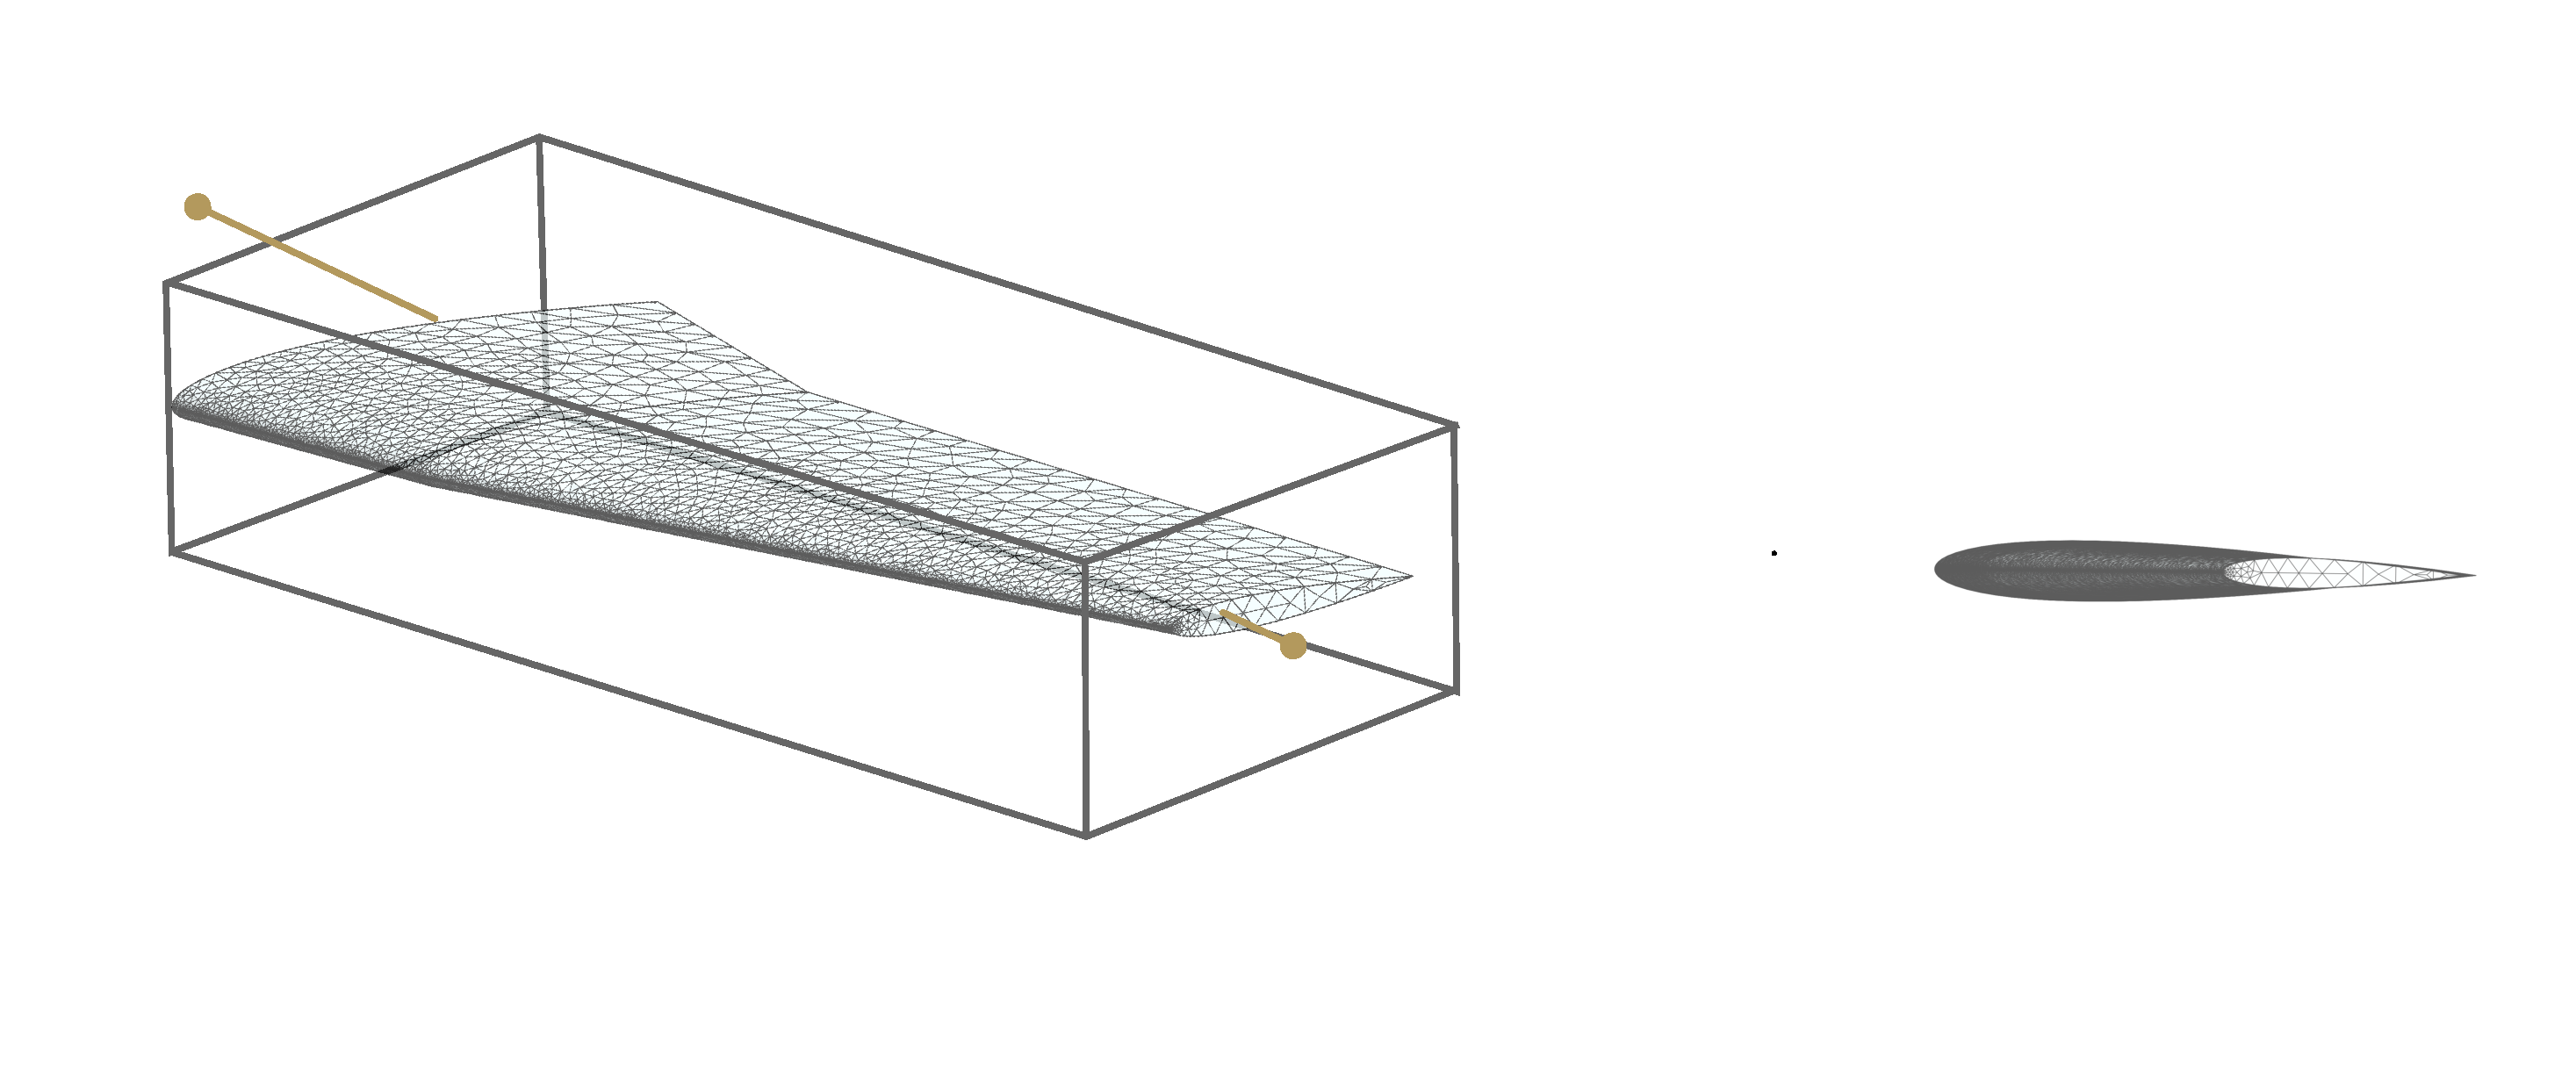
\includegraphics[width=1.0\textwidth]{\mainpath/fig/pdf/sdesign.pdf}
        \caption[Design-model: geometrical approach]{Geometrical approach for the design model as explained in Section~\ref{sec:design_model}. A NACA type airfoil is exemplarily considered here. The airfoil is embedded in a bounding box defined by eight so-called control nodes. The position of these control nodes can be varied, which alternates the shape of the airfoil according to some interpolation functions defined on the nodes. The 24 displacement unknowns are denoted as "abstract shape parameters". Abstract shape variables can be arbitrarily defined. As an example, a rotation axis is defined through the wing. \textbf{REFORMOLATE: With only one independent abstract variable($\alpha$) the whole wing can now be rotated, e.g. to find the optimum angle of attack}}
		\label{fig:sketch_geometrical_approach}
    \end{center}
\end{figure}

\paragraph{Test}
abased
acid
a
SD
acid

%TODO talk about SDESIGN
\subsection{Analysis Model}\label{sec:analysis_model}



The Saddle point formulation of the Lagrangian





%
%%%%%%%%%%%%%%%%%%%%%%%%%%%%%%%%%%%%%%%%%%%%
%% Sensitivity Analysis                    %
%%%%%%%%%%%%%%%%%%%%%%%%%%%%%%%%%%%%%%%%%%%%
%
%\subsection{Aero elastic sensitivity analysis}\label{sec:aeroelastic_sa}
%The \ac{SA} approach applied in this thesis is based on the work of~\cite{Sobieszczanski1990}, for deriving the \ac{GSE} of coupled systems. As introduced by the authors of\cite{Maute2001}, we utilize the three-field formulation of \cite{Farhat1995}.
%
%
%\def\DoptcritJBYabsvarI{\frac{d \optcrit_{j}}{d \absvar_{i}}}
%\def\PoptcritJBYabsvarI{\pdfrac{\optcrit_{j}}{\absvar_{i}}}
%
%\def\PoptcritJBYstructdisp{\pdfrac{\optcrit_{j}}{\structdisp}}
%\def\PoptcritJBYmms       {\pdfrac{\optcrit_{j}}{\mms}}
%\def\PoptcritJBYfstate    {\pdfrac{\optcrit_{j}}{\fstate}}
%
%\def\DstructdispBYabsvarI{\frac{d \structdisp}{d \absvar_{i}} }
%\def\DmmsBYabsvarI       {\frac{d \mms       }{d \absvar_{i}} }
%\def\DfstateBYabsvarI    {\frac{d \fstate    }{d \absvar_{i}} }
%
%The derivative of the optimization criterion~$\optcrit_j$, as introduced in Equation~\eqref{eq:optimization_criteria}, with respect to the optimization variable $\absvar_i$ gives:
%\begin{align}
%\DoptcritJBYabsvarI &=  \PoptcritJBYabsvarI    +
%\PoptcritJBYstructdisp \hleblue{\DstructdispBYabsvarI}  +
%\PoptcritJBYmms        \hleblue{\DmmsBYabsvarI}  +
%\PoptcritJBYfstate     \hleblue{\DfstateBYabsvarI}
%\\
%&=
%\PoptcritJBYabsvarI+
%\T{\begin{bmatrix}
%\PoptcritJBYstructdisp \\[0.5em]
%\PoptcritJBYmms        \\[0.5em]
%\PoptcritJBYfstate     \\[0.5em]
%\end{bmatrix}}
%\cdot
%\begin{bmatrix}
%\DstructdispBYabsvarI \\[0.5em]
%\DmmsBYabsvarI        \\[0.5em]
%\DfstateBYabsvarI     \\[0.5em]
%\end{bmatrix}
%\end{align}
%where the partial derivatives$,\PoptcritJBYstructdisp,\PoptcritJBYmms\text{ and } \PoptcritJBYfstate$ can be directly evaluated within the discretized structure and fluid model through the relation between structural, aerodynamic design and abstract optimization parameters defied in the design model~\ref{sec:design_model}.\\
%The cumbersome part are the derivatives $\DstructdispBYabsvarI,\DmmsBYabsvarI\text{~and~}\DfstateBYabsvarI$
%To obtain them, the governing equations \eqref{eq:3field_basic}\textbf{TODO write down governing equations} have to be derived:
%
%
%
%
%%Differentiation of the governing equations
%\def\PEOSstructBYabsvarI{\pdfrac{\EOSstruct} {\absvar_i}}
%\def\PEOSmeshBYabsvarI  {\pdfrac{\EOSmesh}  {\absvar_i}}
%\def\PEOSfluidBYabsvarI{\pdfrac{\EOSfluid}{\absvar_i}}
%
%\def\PEOSstructBYstructdisp{\pdfrac{\EOSstruct} {\structdisp}}
%\def\PEOSstructBYmms{\pdfrac{\EOSstruct}{\mms}}
%\def\PEOSstructBYfstate    {\pdfrac{\EOSstruct}{\fstate}}
%
%\def\PEOSmeshBYstructdisp{\pdfrac{\EOSmesh}{\structdisp}}
%\def\PEOSmeshBYmms       {\pdfrac{\EOSmesh} {\mms}}
%\def\PEOSmeshBYfstate    {\vec{0}}
%
%\def\PEOSfluidBYstructdisp{\vec{0}}
%\def\PEOSfluidBYmms       {\pdfrac{\EOSfluid} {\mms}}
%\def\PEOSfluidBYfstate    {\pdfrac{\EOSfluid} {\fstate}}
%
%\def\PstructdispBYabsvarI{\pdfrac{\structdisp} {\absvar_i}}
%\def\PmmsBYabsvarI       {\pdfrac{\mms}        {\absvar_i}}
%\def\PfstateBYabsvarI    {\pdfrac{\fstate}     {\absvar_i}}
%
%\begin{align}\label{eq:govering_eqautions_derivative}
%\def\arraystretch{2.0}
%\begin{bmatrix}
%\PEOSstructBYabsvarI \\[0.5em]
%\PEOSmeshBYabsvarI   \\[0.5em]
%\PEOSfluidBYabsvarI
%\end{bmatrix} +
%  \underbrace{\begin{bmatrix}
%  \PEOSstructBYstructdisp & \PEOSstructBYmms & \PEOSstructBYfstate \\[0.5em]
%  \PEOSmeshBYstructdisp   & \PEOSmeshBYmms   & \PEOSmeshBYfstate   \\[0.5em]
%  \PEOSfluidBYstructdisp  & \PEOSfluidBYmms  & \PEOSfluidBYfstate
%  \end{bmatrix}}_{\tensor{A}}
%    \hleblue{\begin{bmatrix}
%    \PstructdispBYabsvarI \\
%    \PmmsBYabsvarI        \\
%    \PfstateBYabsvarI     \\
%    \end{bmatrix}} = \vec{0}
%\end{align}
%In this equations $\textstyle{\PEOSstructBYabsvarI}$ and $\textstyle \PEOSfluidBYabsvarI$ can be again directly evaluated using the relation specified in the design model. The matrix of first derivatives~$\tensor{A}$ is from now on denoted as the "Jacobian of the optimization problem".
%\\
%Combining the previous two equations, it follows that the total derivative of the optimization criterion with respect to the abstract variables can be expressed as:
%\begin{align}\label{eq:totderiv_optcritBYabsvar}
%\DoptcritJBYabsvarI = \PoptcritJBYabsvarI -
%\underbrace{\T{\begin{bmatrix}
%\PoptcritJBYstructdisp \\[0.5em]
%\PoptcritJBYmms        \\[0.5em]
%\PoptcritJBYfstate     \\[0.5em]
%\end{bmatrix}}}_{n_{\optcrits}\times n_{eq}}
%  \underbrace{\inv{\tensor{A}}}_{n_{eq}\times n_{eq}}
%  \underbrace{\begin{bmatrix}
%  \PEOSstructBYabsvarI \\[0.5em]
%  \PEOSmeshBYabsvarI   \\[0.5em]
%  \PEOSfluidBYabsvarI
%  \end{bmatrix}}_{n_{eq}\times n_{\absvars}}
%\end{align}
%
%\subsubsection{Direct vs. adjoint approach}
%Equation~\ref{eq:totderiv_optcritBYabsvar} suggests, that there are two alternatives to compute vector-matrix-vector product above.\\
%
%\paragraph{Direct approach}
%Firstly, one could first compute the derivatives of the aeroelastic response for each abstract variable and perform the matrix product with $\tensor{A}$:
%
%\begin{align}\label{eq:direct_approach}
%\begin{bmatrix}
%\DstructdispBYabsvarI \\[0.5em]
%\DmmsBYabsvarI   \\[0.5em]
%\DfstateBYabsvarI \\[0.5em]
%\end{bmatrix}
%&=
%  -\inv{\tensor{A}}
%  \begin{bmatrix}
%  \PEOSstructBYabsvarI \\[0.5em]
%  \PEOSmeshBYabsvarI   \\[0.5em]
%  \PEOSfluidBYabsvarI
%  \end{bmatrix}
%\text{~~~and then}\\
%\DoptcritJBYabsvarI &= \PoptcritJBYabsvarI -
%\T{\begin{bmatrix}
%\PoptcritJBYstructdisp \\[0.5em]
%\PoptcritJBYmms        \\[0.5em]
%\PoptcritJBYfstate     \\[0.5em]
%\end{bmatrix}}
%  \begin{bmatrix}
%  \DstructdispBYabsvarI \\[0.5em]
%  \DmmsBYabsvarI   \\[0.5em]
%  \DfstateBYabsvarI \\[0.5em]
%  \end{bmatrix}
%\end{align}
%Where the total complexity can be approximated as $\order{n_{eq}^2n_{\absvars}+n_{\optcrits}n_{eq}n_{\absvars}}$
%
%
%
%\paragraph{Adjoint approach}
%Secondly, one could also first compute the derivatives of the optimization criteria and multiply with the Jacobian before substituting this into Equation~\eqref{eq:totderiv_optcritBYabsvar}:
%\begin{align}\label{eq:firststep_adjoint}
%\begin{bmatrix}
%\adjoints_{\structdisp} \\
%\adjoints_{\mms}        \\
%\adjoints_{\fstate}
%\end{bmatrix}&=
%  \tensor{A}^{-T}
%  \begin{bmatrix}
%  \PoptcritJBYstructdisp \\[0.5em]
%  \PoptcritJBYmms        \\[0.5em]
%  \PoptcritJBYfstate     \\[0.5em]
%  \end{bmatrix}
%\\
%\DoptcritJBYabsvarI &= \PoptcritJBYabsvarI -
%\T{\begin{bmatrix}
%\adjoints_{\structdisp} \\
%\adjoints_{\mms}        \\
%\adjoints_{\fstate}
%\end{bmatrix}}_j
%  \begin{bmatrix}
%  \PEOSstructBYabsvarI \\[0.5em]
%  \PEOSmeshBYabsvarI   \\[0.5em]
%  \PEOSfluidBYabsvarI
%  \end{bmatrix}
%\end{align}
%Where the total complexity can be approximated as $\order{n_{eq}^2n_{\optcrits}+n_{\optcrits}n_{eq}n_{\absvars}}$\\
%
%
%If one or the other approach is to be preferred depends in on the optimization setup, particularly the number of optimization criteria and the number of optimization variables. Looking at the orders above, one can conclude that if the number of abstract parameters $n_{\absvars}$ is smaller than the number of optimization criteria, the direct approach is more efficient, otherwise the adjoint approach is to be preferred. Additionally the on can argue, that the relevant term in the orders above is the one with $n_{eq}^2$  since it dominates the sum.
%
%
%\section{Direct Sensitivity Analysis for the Euler equations}\label{sec:direct_sa}
%
%
%The A matrix for the direct approach in ALE formulation looks like
%\def\AoneoneALE{\stiffmat}
%\def\AonetwoALE{\pdfrac{\sload}{\mms}}
%\def\AonethreeALE{\pdfrac{\sload}{\fstate}}
%
%\def\AtwooneALE{\begin{bmatrix}
%                \stiffmat_{\Omega \Gamma} \ifaceprojStoF \\
%                \ifaceprojStoF
%                \end{bmatrix}
%               }
%\def\AtwotwoALE{
%               \begin{bmatrix}
%               \stiffmat_{\Omega \Omega} & \vec{0}  \\
%               \vec{0}                   & \dmat{I}
%               \end{bmatrix}
%               }
%\def\AtwothreeALE{\vec{0}}
%
%\def\AthreeoneALE{\vec{0}}
%\def\AthreetwoALE{\pdfrac{\dmat{F}_2}{\mms_\Omega}}
%\def\AthreethreeALE{\jactwo}                       %TODO find better shortcurt name
%\begin{align}\label{eq:Amatrix_ALE}
%\tensor{A}=
%\begin{bmatrix}
%  \PEOSstructBYstructdisp & \PEOSstructBYmms & \PEOSstructBYfstate \\[0.5em]
%  \PEOSmeshBYstructdisp   & \PEOSmeshBYmms   & \PEOSmeshBYfstate   \\[0.5em]
%  \PEOSfluidBYstructdisp  & \PEOSfluidBYmms  & \PEOSfluidBYfstate  \\[0.5em]
%\end{bmatrix}=
%  \begin{bmatrix}
%  \AoneoneALE    &  \AonetwoALE    &  \AonethreeALE  \\[0.5em]
%  \AtwooneALE    &  \AtwotwoALE    &  \AtwothreeALE  \\[0.5em]
%  \AthreeoneALE  &  \AthreetwoALE  &  \AthreethreeALE
%  \end{bmatrix}
%\end{align}
%Where, $\AthreethreeALE$ is the Jacobian of the second order row flux. It shall be noted that constructing this Jacobian is not a trivial issue and takes up a lot of computational resources, especially for \ac{FV}, as described in \cite{Farhat1995}. Investigation into whether this term can be approximated at first order were carried out in \cite{Maute2001} and \cite{Maute2003}.\\
%Furthermore, \cite{Piperno2000} considered replacing the two mesh motion related matrices $\AonetwoALE$ and $\AthreetwoALE$ by a transpirational boundary condition. The consequences of this approach are also investigated in \cite{Maute2001} and \cite{Maute2003}.\\
%This thesis, however, dow not use any of this simplifications.
%~\\
%The derivation of the sensitivities, can be achieved in a staggered scheme, very similar to the one, described in \ref{sec:3field}\textbf{TODO}. It consists of five steps.
%
%\paragraph{1) Update the structural displacement sensitivity to a new time step}
%BY differentiating equations~\eqref{eq:3field_structure} and \eqref{eq:eos_struct} and applying an under relaxation, we can obtain
%\begin{align}\label{eq:underrelax_structdisp}
%\tfrac{\its{\structdisp}}{\absvar_i} =
%(1-\theta)
%\tfrac{\its{\structdisp}}{\absvar_i} +
%\theta \tfrac{\fic{\structdisp}}{\absvar_i}
%\end{align}
%
%where $\fic{\structdisp}$ is obtained from:
%\begin{align}\label{eq:fictious_structdisp}
%\stiffmat \tfrac{\fic{\structdisp}}{\absvar_i} =
%\pdfrac{TODO}{\absvar_i} + \pdfrac{\its{\ifaceprojStoF}}{\absvar_i} -
%\pdfrac{\stiffmat}{\absvar_i} \structdisp
%\end{align}
%
%
%\paragraph{2) Transfer sensitivity of structure motion to the interface}
%\begin{equation}\label{eq:interface_projections}
%\tfrac{\its{\structdisp}_T}{\absvar_i} =
%\ifaceprojStoF \tfrac{\its{\structdisp}}{\absvar_i}
%\end{equation}
%
%
%\paragraph{3) Compute derivative of fluid mesh motion}
%The fluid mesh motion is computed by solving the pseudo Dirichlet problem as described in~\cite{Farhat1995}. By design, the fictions stiffness matrix $\fic{\stiffmat}$ does not depend on the abstract optimization variables $\absvars$
%\begin{align}\label{eq:mms_domain}
%\fic{\stiffmat}_{\Omega \Omega}  \tfrac{\its{\mms}_{\Omega}}{\absvar_i} =
%-\fic{\stiffmat}_{\Omega \Gamma} \tfrac{\its{\mms}_{\Gamma}}{\absvar_i}
%\end{align}
%with
%\begin{align}
%\tfrac{\its{\mms}_{\Gamma}}{\absvar_i} =
%\tfrac{\its{\mms}_{\Gamma}}{\absvar_i}
%\end{align}
%
%
%\paragraph{4) Compute the sensitivity of the fluid state variables}
%The derivatives of the fluid state variables are computed by
%\begin{align}
%\jactwo \tfrac{\itss{\fstate}}{\absvar_i} =
%\pdfrac{\tensor{F}_2}{\absvar_i} - \pdfrac{\tensor{F}_2}{\mms} \its{\tfrac{\mms}{\absvar_i}}
%\end{align}
%
%\paragraph{5) Compute the sensitivity of the structure load vector}
%The derivative of the fluid load with respect to the abstract variables can be computed by the third of Equations~\eqref{eq:direct_approach} with the definition of $\tensor{A}$ as specified in \eqref{eq:Amatrix_ALE}.
%\begin{align}\label{eq:deriv_floadBYabsvar}
%\pdfrac{\itss{\fload}}{\absvar_i} =
%\pdfrac{\itss{\fload}}{\mms}    \tfrac{\its{\mms}}   {\absvar_i} +
%\pdfrac{\itss{\fload}}{\fstate} \tfrac{\its{\fstate}}{\absvar_i}
%\end{align}
%
%and compute project it onto the structure via
%\begin{align}
%\pdfrac{\itss{\sload}}{\absvar_i} = \ifaceprojFtoS \pdfrac{\itss{\fload}}{\absvar_i}
%\end{align}
%~\\
%~\\
%The convergence of the staggered algorithm can be monitored via
%\begin{align}
%\begin{split}
%  \norm{ \stiffmat \tfrac{ \itss{\fic{\structdisp}} }{\absvar_i}  -  \pdfrac{TODO}{\absvar_i} - \pdfrac{\itss{\sload}}{\absvar_i}  +  \pdfrac{\stiffmat}{\absvar_i}}_{2} &
%  \leq \\
%  \tolsa \norm{ \stiffmat \tfrac{ \itn{\fic{\structdisp}}  }{\absvar_i}  -  \pdfrac{TODO}{\absvar_i} - \pdfrac{\itn{\sload}}{\absvar_i}  +  \pdfrac{\stiffmat}{\absvar_i}}_{2} &
%\end{split} &
%\\
%\begin{split}
%  \norm{\jactwo \tfrac{\itss{\fstate}}{\absvar_i} + \pdfrac{\tensor{F}_2}{\absvar_i} + \pdfrac{\tensor{F}_2}{\mms} \itss{\tfrac{\mms}{\absvar_i} }   }_{2} &
%  \leq \\
%  \tolsa \norm{\jactwo \tfrac{\itn{\fstate}}{\absvar_i} + \pdfrac{\tensor{F}_2}{\absvar_i} + \pdfrac{\tensor{F}_2}{\mms} \itn{\tfrac{\mms}{\absvar_i} }   }_{2} &
%\end{split} &
%\end{align}
%
%
%\section{Adjoint Sensitivity analysis for the Euler equations}\label{sec:adjoint_sa}
%The adjoint SA follows the same scheme as the direct one
%
%
%Equation \eqref{eq:firststep_adjoint} can be written as:
%\def\AonetwoALEadjoint{\begin{bmatrix}
%                \pdfrac{\sload}{\mms_\Omega}
%                \pdfrac{\sload}{\mms_\Gamma}
%                \end{bmatrix}             }
%
%\def\AthreetwoALEadjoint{\begin{bmatrix}
%                  \pdfrac{\dmat{F}_2}{\mms_\Omega}
%                  \pdfrac{\dmat{F}_2}{\mms_\Gamma}
%                  \end{bmatrix}                   }
%                  
%\def\PoptcritsBYstructdisp{\pdfrac{\optcrits}{\structdisp}}
%
%\begin{align}\label{eq:adjoint_equation}
%\T{\begin{bmatrix}
%\AoneoneALE    &  \AonetwoALEadjoint    &  \AonethreeALE  \\[0.5em]
%\AtwooneALE    &  \AtwotwoALE    &  \AtwothreeALE  \\[0.5em]
%\AthreeoneALE  &  \AthreetwoALEadjoint  &  \AthreethreeALE
%\end{bmatrix}}
%  \begin{bmatrix}
%  \vec{a}_{\structdisp} \\
%    \begin{bmatrix}
%    \vec{a}_{\mms_\Omega} \\
%    \vec{a}_{\mms_\Gamma} \\
%    \end{bmatrix}       \\
%  \vec{a}_{\fstate}     \\
%  \end{bmatrix}
%  =
%    \begin{bmatrix}
%    \PoptcritJBYstructdisp \\
%      \begin{bmatrix}
%      \pdfrac{\optcrits}{\mms_\Omega} \\
%      \pdfrac{\optcrits}{\mms_\Gamma} \\
%      \end{bmatrix}        \\
%    \PoptcritJBYfstate     \\
%    \end{bmatrix}
%\end{align}
%\textbf{TODO} check if the index j is really required here!
%A stated earlier, the matrices $\pdfrac{\optcrits}{\mms}$ and $\pdfrac{\optcrits}{\fstate}$ can be computed analytically. As for $\AthreethreeALE$, we follow the methodology outlined in \cite{Lesoinne2001} for evaluating ans storing it efficiently as the product of flux operators. Again the staggered procedure for solving the adjoint state problem shares the same computational kernels with the partitioned aeroelastic scheme described in~\cite{Farhat1995}\\
%
%\paragraph{1) Update the adjoint structure displacement to the new time step}
%\begin{align}
%\itss{\structdispad}=(1-\theta)\its{\structdispad}+\theta \itss{\fic{\structdispad}} \\
%\end{align}
%where $\itss{\fic{\structdispad}}$ is obtained from
%\begin{align}
%\stiffmat \itss{\fic{\structdispad}} = \PoptcritsBYstructdisp - \stiffmat_{\Omega\Gamma} \ifaceprojStoF \its{{\mmsad}_{\Omega}} + \ifaceprojStoF \its{{\mmsad}_{\Gamma}}
%\end{align}\textbf{TODO derive this equation}
%
%\paragraph{2) Compute the adjoint fluid state by solving}
%\begin{align}
%\T{\jactwo} \itss{\fstatead} = \pdfrac{\mms}{\fstate}+ \pdfrac{\sload}{\T{\fstate}} \itss{\structdispad}
%\end{align}\textbf{TODO derive this equation}
%Again, $\pdfrac{\optcrits}{\fstate}$ is computed analytically from the relations defined in the design and aeroelastic model.
%
%
%\paragraph{3) Compute adjoint mesh motion in domain and on the interface}
%\def\PoptcritsBYfstate{\pdfrac{\optcrits}{\fstate}}
%\begin{align}
%\fic{\stiffmat}_{\Omega\Omega} \itss{{\mmsad}_{\Omega}} =
%\pdfrac{\optcrits}{\mms_\Omega} -
%\pdfrac{\sload}{\mms_\Omega} \itss{\structdispad} -
%\pdfrac{\T{\dmat{F}_1}}{\mms_\Omega} \itss{\mmsad}\text{ in }\Omega
%\end{align}\textbf{TODO check equations}
%And the adjoint mesh motion on the interface is computed as $\itss{{\mmsad}_{\Gamma}}$
%\begin{align}
%\itss{{\mmsad}_{\Gamma}} =
%\pdfrac{\optcrits}{\mms_{Gamma}} +
%\pdfrac{\sload}{\mms_\Gamma} \itss{\structdispad}    -
%\T{\pdfrac{\dmat{F}_2}{\mms)_\Gamma}}\text{ on }\Gamma
%\end{align}
%where $\PoptcritsBYfstate$ is computed analytically.
%~\\
%~\\
%The convergence of the staggered adjoint optimization algorithm can be monitored via
%\begin{align}
%\norm{\vec{R}_{\optcrits}-
%\T{\tensor{A}} \itss{\vec{a}} }
%\leq
%\tolsa\norm{\vec{R}_{\optcrits}}
%\end{align}



\end{document}
